
\begin{center}\texttt{2 - Agile, introduction}\end{center}
\hrulefill \\

\noindent Began as a movement of senior devs who questioned the traditional Software Engineering methodologies, considered no longer suitable for contemporary needs. That type of hierarchical, strict and traditional approach takes the name of \textbf{command-and-control.}

 Agile is basically a set of methods and techniques and how you should use those.

 \noindent Key points of the Agile approach are:
 \begin{itemize}
     \item there is no longer a central figure of ``Project Manager'', i.e. one person who establishes the planning of all activities. Agile approach values team cooperation in spite of a central authority;
     \item Change must be welcomed instead of dreaded, in software and all artefacts - change is unavoidable and it's usually a change for the better, for a product that the customer will like better. Software is ``ethereal'', unlike many other products and goods, therefore requirements are difficult to identify straight away, change should thus be especially welcome.
     \item focus on the code rather than on the documentation and models. Quality strongly depends on people (many things strongly depend on people, as we will find out).
 \end{itemize}

\noindent Goals and ``promises'' of Agile: more effective \& efficient work, make better decisions, higher product quality, happier customer, less work hours, on-time deliveries.

 \noindent The Agile mindset, based on ideas, values and principles:
 \begin{itemize}
     \item if you're Agile, you are willing to share knowledge - no competition through keeping knowledge to yourself;
     \item TEAM before INDIVIDUALS!;
     \item everyone takes responsibility for decisions and stuff, thus there is more commitment from all the team members. Everyone is invested in the project and wants to see it finished;
 \end{itemize}

If you have a Manager figure in your team, you are not Agile. There might be, of course, a manager in the \textit{company}, but not in the project team.

\noindent Different approaches during a daily stand-up meeting:
\begin{itemize}
    \item Agile: people cooperating;
    \item non-Agile: Manager making a checkpoint;
\end{itemize}

Agile values:
\begin{itemize}
    \item working software over documentation: delivering artefacts doesn't necessarily equal to progress! There will be some documentation, but it no longer matters as much as in the Waterfall-like models;
    \item people over processes: individuals and interactions are important, it is okay to compromise over processes and tools. The willingness to carry out a prj depends much more on the people than on the processes;
    \item respond to changes over following a plan:
    \item customer collaboration over contract negotiation. Contracts in this context are more of an evolving negotiation rather than a final thing that remains unchanged for the whole prj $\rightarrow$ the customer will have to continuously cooperate and give feedback in Agile approach;
\end{itemize}

The main limitation of the Waterfall model is that requirements must be defined as completely as possible at the very beginning of the project and they are never changed during further steps of the process: this doesn't welcome change, this doesn't even \textit{contemplate} change at all, and it's not suitable for any kind of project that is innovative.

\noindent Better-than-not-doing-it phenomenon: in an attempt at transitioning to Agile, you adopt agile methodologies without actually \textit{being} Agile - going agile is not equal to becoming an agile team. Becoming Agile entails embracing the values and principles of Agile. Often times this results in an improvement of individual skills but not in growth as a team (doesn't sound very Agile to me);

\noindent Although it may sound counter-intuitive, in Agile you actually do more planning than you'd do in traditional approaches, the main difference lies in \textit{when} and \textit{which kind} of planning you do, and what you include in it.


Sometimes it happens that only some people in the team will have Agile methodologies, though that is rare because eventually that leads to frictions and it's hard to align everyone.

 \noindent Again, Agile is about the mindset - thus, you don't necessarily have to adopt Scrum, XP, or any Agile methodology to be Agile. In some cases, with enough expertise, you might come up with your own methodology.


\noindent Agile methods divided in 4 main categories:
\begin{enumerate}
    \item delivery of the product:
    \begin{enumerate}
        \item deliver, early and continuously, valuable software to satisfy the customer. It's the best way to get customer cooperation and it has highest priority;
        \item welcome change, because the aim is to give the customer a valuable product that satisfies their requests. To ease the welcoming and application of changes, there are several development toolchains that help refactor and change our product safely without messing up the rest of the features and stuff. Change is not bad, change is normal and a good discovery, not to be necessarily associated with anyone's mistake;
        \item don't just deliver frequently, but also in a precise timeframe! Establish 2 weeks, or 4, as long as the iteration is time-boxed, preferably small boxes bc it's good for the customer to verify the work and give feedback after seeing a demonstration of it (it's also good for Risk management btw, gives better insight on what works what doesn't). Note that iterations don't have to keep the same length over the course of the project, often times they start shorter and become longer after the requirements and features are outlined more precisely;
    \end{enumerate}
    \item communication (how to organize activities): 
    \begin{enumerate}
    \item prefer face-to-face communication;
    \item business people and developers must work together daily throughout the project;
    \item start motivated and stay motivated! Productivity comes from cooperation, not competition. No CYA attitude (cover-your-ass, avoiding holding responsible for your actions, maybe trying to shift blame on someone else), no individual awarding;

    \end{enumerate}
    \item execution (how to perform activities):
    \begin{enumerate}
        \item Working software is the primary measure of progress;
        \item no changing the workload, all paces should be constant (I guess against crunching);
        \item attention to technical excellence and good design enhances agility;
    \end{enumerate}
    \item improvement (project and team):
    \begin{enumerate}
        \item avoid enlarging the project unnecesarily;
        \item there's no team manager or any type of exclusive role, everyone works on everything (team is self-organizing);
        \item regularly reflect on how to become more effective and learn from bad outcomes. Change doesn't imply that a mistake has occurred and needed fixing, but you can still learn something from it.
    \end{enumerate}
\end{enumerate}

\newpage
\noindent \underline{Scrum} - the most widely used Agile methodology.

 \noindent Core values:
 \begin{itemize}
     \item courage: members should stand up for the project;
     \item commitment: willingness to make decisions for the project;
     \item respect: well, respect for everyone's work;
     \item focus: people working on a project don't usually work on any other in the meantime;
     \item openness: very important for detecting and dealing with problem. Everyone's work is accessible to everyone - zero secrecy policy;
 \end{itemize}

Three main roles in a Scrum project team (each with different skills and competences):
\begin{enumerate}
    \item Project Owner (PO): interacts and commits to the customer, keeps a Product Backlog (PB). It's the main contributor to Requirements, writes user stories and puts them in the Product Backlog. Motivates the team by defining the goals of the project; Prioritizes the items in the PB based on what the customer expects to be done by a given deadline;
    \item Scrum Master (SM): just a Scrum expert. Doesn't actively work at the project, only monitors the team to make sure that they are applying the Scrum methodology appropriately. The SM is also the figure in charge of defending the team in case the PO comes up with unrealistic requests and expects too much from the TMs;
    \item Team Members (TM): those who work on the feature, the devs, typically.
\end{enumerate}

Scrum is an incremental iterative approach, iterations take the name of \textit{``Sprints''}: typically 3-4 weeks long and timeboxed. The team (PO + SM + TM) partakes in \textit{at least} one meeting every day, a quick one that lasts no more than 15-20 minutes. The methodology strongly relies on the concept of User Stories, which are basically simplified requirements that specify the feature and reason for usage that a stakeholder/user might want to see in the product.

 \noindent Each sprint has its own Sprint Backlog, a subset of the PB that consists of the features the team will be working on for this one sprint.

\begin{figure} [H]
    \centering
    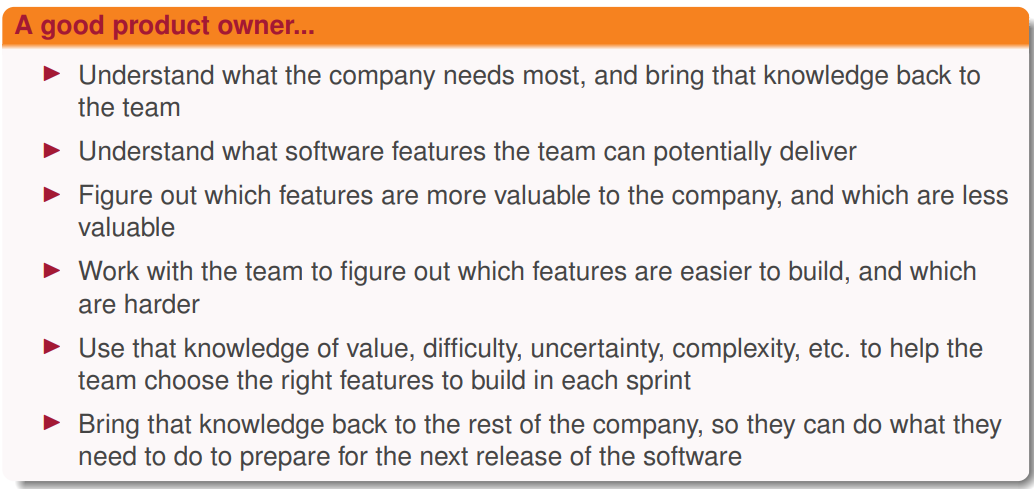
\includegraphics[scale=0.5]{Figures/02/po_resp.png}
    \caption{PO responsibilities}
    \label{fig:poresp}
\end{figure}

\noindent Building the Scrum team:
\begin{itemize}
    \item you want $5\div7$ people, + SM + PO;
    \item Don't try to adapt people to the project - seek people who are committed to the way you work in Agile; that also applies to the management roles, mgmt people should also be aware of the Agile methodology, so that they won't be pushing the team to behave in non-Agile behavior, i.e. Waterfall;
    \item Team members must share the same \textbf{vision} on the prj!
    \item Create, communicate and empower the vision of the project, i.e. how the future will change;
    \item set achievable short-term goals;
    \item be persuasive (wow).
\end{itemize}

\noindent Team Members are multitalented: everyone can do a bit of everything;

 \noindent Consultants are optionally summoned as experts of a specific domain, they join the team for a single sprint so they are usually less of a team player and more of an expert lone wolf; at any rate, the team is usually happy to have consultants on board, because they bring opportunities to learn from their expertise.

\noindent Sprints:
\begin{itemize}
    \item duration: $2\div4$ weeks, or a month. Cannot be stopped unless in case of emergency;
    \item timeboxed: the duration is fixed!!
    \item it starts with a meeting where the team decides ``what to do'': if the team agrees that they won't be able to meet the promised commitments to customer, they proceed to tell the PO asap, the PO will tell the customer;
    \item The Product Backlog is always visible to everyone - it's a 3 column table with To-Do, in progress and Done Stories;
    \item end activities, ``closing/review'' meeting: all members and all stakeholders participate (approx 30 min duration). Goal: demonstrate the product by means of the prototype, no slides (no preparation either)! Customer tries it first-hand and gives feedback. PO optionally updates the PB;
    \item Retrospective meetings are held by the SM after the end of the Sprint: Team reflects on the last sprint, what went well, what didn't, where to improve;
\end{itemize}

\noindent Day 1 of the new Sprint, Planning activities (TM + SM + PO:
\begin{itemize}
    \item 1st part (4hr, Exploration): the goal is to prioritize the elements in the PB to complete this time, resulting in a new Sprint Backlog;
    \item 2nd part (4hr, Operative plan): assign individual tasks to each member;
\end{itemize}

\noindent How long should a sprint last? Depends on a lot of things: customer availability to meet the team; how often feedback is required; how long is the whole prj and what phase we're on; whether the team has preferences.

 \noindent User Stories:
 \begin{figure}[H]
     \centering
     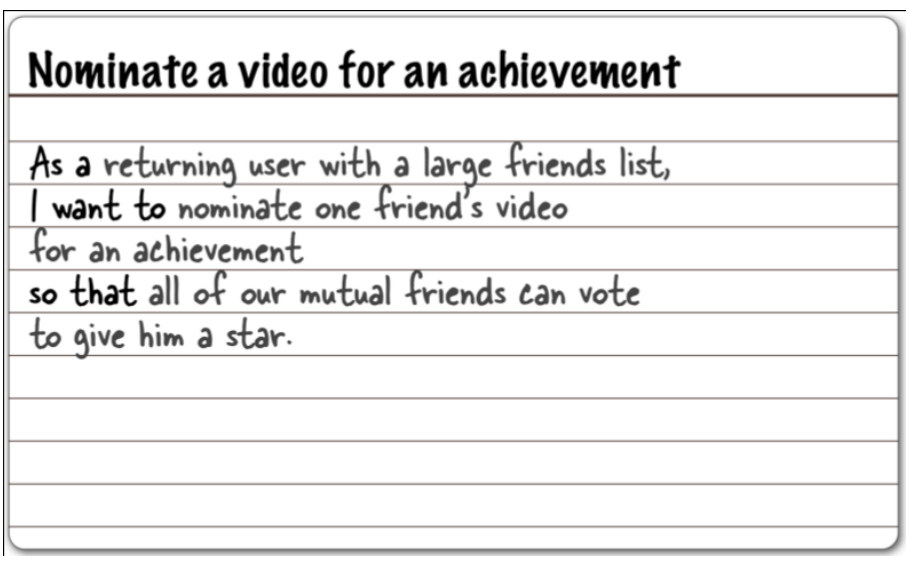
\includegraphics[scale=0.4]{Figures/02/usrstories.png}
     \caption{User story. Comes with satisfaction conditions (multiple)}
     \label{fig:us1}
 \end{figure}

\noindent Main tool for defining functional requirements. Describe usage of system and goal of some user. To determine how complex the requirement of the story is, the team gives it a score: Story Points. TMs + PO should converge to agree on the scores eventually: for that, they discuss or play Planning Poker. With this, the team makes very important decisions for the prj, but it's generally a good strat: it's simple, it's based on reliable opinions of the team rather than the managers, plus the team communicates during these operations, improving commitment. User Stories shouldn't be too specific nor too broad in the behavior they describe, but of the right granularity.\\Velocity: nr of story points delivered during a sprint: you want to deliver story points $\leq$ your velocity. Initially, the team estimates a value for the velocity - afterwards they will estimate velocity through past history.

\noindent Second meeting of the sprint (duration: 1 hr per sprint week): SM takes user stories, the team discuss possible tasks to accomplish it; each task is written on a card, each task should take around 2 days to complete; discussed USs and tasks are added to the Sprint backlog, we'd like to have them all completed at the end of the sprint (bc we promised the customer)

 \noindent Three levels of complexity: Epics, Themes, Stories
 \begin{itemize}
     \item many Stories form a Theme, many Themes form an Epic;
     \item rule of thumb: user stories should describe the smallest action a user does to achieve a goal - ``redesign the UI'' is a goal way too large to fit in a Story, it's more of an Epic;
     \item Time To Complete: tasks - 2 days; stories - no more than a Sprint; Themes - more than a Sprint; Epics - several sprints.
 \end{itemize}

 Day 2 of the sprint - the implementation begins. Pick up a task, make sure to tell the team you picked it, move it to the 2nd column ``in Progress''. When ALL the tasks of a Story are done, the PO might decide to move the Story to Done (DONE DONE = ready to be demonstrated). Things that were not completed by the end of the Sprint, will be considered To-Do in the next one's PB.

 \noindent Burndown Chart:
\begin{figure} [H]
    \centering
    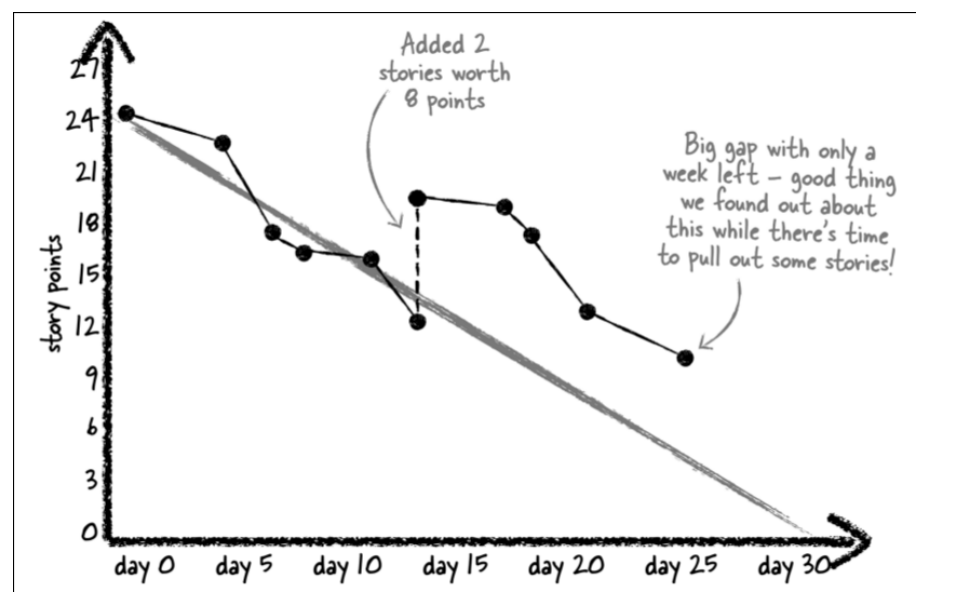
\includegraphics[scale=0.4]{Figures/02/bdc.png}
    \caption{Burndown chart: progress monitoring tool. Straight line is the ideal progress. The spike on day 13 is an exceptional situation, the customer changes what they want to be done mid-sprint.}
    \label{fig:bdc}
\end{figure}

\noindent Daily Stand-Up meeting: fast, 15-minute meeting like at the vending machine. The team catches up on what they did and what they're up to today, what hardships today might bring. Everyone submits issues for further reflection, won't discuss them yet tho. The PO doesn't really partake in these conversation, but will clarify in case of need. Based on what you hear from the rest of the team, you will make some decisions $\rightarrow$ Last Responsible Moment: the moment of highest knowledge of the situation - this is the moment when you're as knowledgeable as it gets to make some decision, thus you can make a wise one. Listen, stay humble, cooperate. It's important that everyone participates - it's best if a different team member starts the conversation each time.

\noindent Last day of Sprint: Sprint Review (duration: 1hr per sprint week). The customer attends. Objective: show what you did, get feedback and POV of customer. It's important to be honest with the customer and don't make up features that you don't actually have ready. Negative surprises are more dangerous WRT a Waterfall prj, because the contract with the customer is monthly, so they might not renew it upon multiple disappointments. Demo is a validation tool, not a way to be criticized by the customer, perceive it as a chance to find errors and changes needed.

\noindent Retrospectives: the very last meeting of the Sprint (no customer in here). Duration: 30 min per sprint week: mostly it's an occasion in which everyone proposes topics of discussion in order to learn and improve for the next sprint.

\newpage\noindent \underline{eXtreme Programming (XP)} - Iterative approach

 \noindent Main drive: Making the welcoming of changes as easy as possible, even in late stages of the prj.

\noindent XP Practices:
\begin{itemize}
    \item Programming:
    \begin{itemize}
        \item Test-First Programming: first write the tests, then write the code in order to pass the tests;
        \item Pair Programming: assign two programmers to work on the same code, literally on the same keyboard in turns (one codes one observes). Promotes cooperation and interaction, an innovative approach, also bc pairs are mixed from iteration to iteration. Seems costly to assign 2 people on the same task, but it saves money on the long run due to less errors and such;
        \item Incremental Design: prioritize big decisions in the early stages, keep making decisions over the course of the development + avoid duplication as much as possible $\rightarrow$ more flexible and easy-to-change software;
    \end{itemize}
    \item Integration:
    \begin{itemize}
        \item Building the prj (including all tests and relative test results) should take no longer than 10 minutes so you can do it more than once a day and check new stuff more easily;
        \item no ``big bang'' integrations once a day, they might block the progress of the whole team, it might introduce many issues to fix. Rather commit small changes and often. Use Build Tokens (the chicken toy lol) to establish who gets to merge their progress to the central branch, in order to avoid conflicts and inconsistencies everywhere; 
    \end{itemize}
    \item Planning:
    \begin{itemize}
        \item delivery of software only when in status DONE DONE - unlike Scrum, there's no PO who checks the requirements, here it's about all tests passing;
        \item super fast iterations (1 week!), no PO but direct interaction with the customer;
        \item Quarterly cycles: used in XP to do long-term planning, happens once every 3 months. Make reflections on the state of things, what to learn and improve etc., there's no time for that in XP's short iterations;
        \item Slack: same thing as scrum, low-priority stories that are added to every weekly cycle. Stories that are not too relevant but still useful, if you have any time left before the end of the cycle, you tackle those. Refactoring code is a good example of slack activity;
    \end{itemize}
    \item Team:
    \begin{itemize}
        \item Face-to-face communication is much preferred to passing documents (applies to all things Agile in general);
        \item you should have a space to practice individual reflection and a space to sit together and interact with the others. Try to favor both activities. Informative workspace is a place where you can find prj info all around - whiteboards and stuff! It's there, it's immediate, information radiators making osmotic communication (you get the info simply by being there, no need to go searching);
        \item Energized work: no crunching, give the team enough time to work on everything in normal pace and time. Avoid distractions, when you work you work, ez;
        \item Whole team: the team produced the software, all together with the same objective. No specialists in the team, everyone does everything.
    \end{itemize}
\end{itemize}

\noindent XP values:
\begin{itemize}
    \item Communication: everyone is aware of everything;
    \item Simplicity: always favor the easiest, simplest solutions possible;
    \item Feedback: together with testing, ensures the quality of the product;
    \item Courage: to refactor big portions of the code, to make choices;
    \item Respect: each team member brings value, trust the others and their skills.
\end{itemize}

\noindent Humanity: take care of people; Economics: keep budget in mind; Mutual Benefit: balance benefit to individuals team and customer; Self-Similarity: try sticking to a winning strat in different contexts; Improvement: do ur best; Diversity: different opinion make the prj better!; Reflection: team is aware of what works and what doesn't; Flow: constant devpm and delivery; Opportunity: given by problems! to learn; Redundancy: helps to avoid trouble; Failure: yea it's OK; Quality: doesn't help to deliver quick and well; Accepted resp.ty: i.e. make decisions; Baby Steps: in the right direction :D

\noindent Charge for usage, not for development: customer doesn't pay for my dev., but for how much they're going to use of the project. Optimized feedback! Customer will be prone to giving good feedback on what they exactly want to see implemented.

\noindent Technical debt: every time you make a decision, implement stuff, you take into account a debt that consists in refactoring hours, pretty much. Fail fast strategy reduces risk of accumulating debt. Debt is the difference between perfect, ideal code and what you actually have - you do that through refactoring.

%ITS NOT IMPOSSIBLY DIFICULT KEEP GOINGGGGGGGGGGGGGGGG 